\cref{fig:sec-gen-intro-mt:mt} illustrates different types of model transformations.
In general, a model transformation $\MT\colon \Lang(D_1) \TransMT \Lang(D_2)$ is a relation that maps (transforms) models $M \in \Lang(D_1)$ in a domain-specific modelling language (DSL) $\Lang(D_1)$ in source domain $D_1$ (in)to models $M' \in \Lang(D_2)$ in DSL $\Lang(D_2)$ in target domain $D_2$ \cite{Mens2006125}.
Therefore, $(M,M') \in \MT$ means that model $M$ expressed in modelling language $\Lang(D_1)$ is transformed into model $M'$ expressed in modelling language $\Lang(D_2)$ via model transformation $\MT$.
The model transformation is exogeneous if lanuage $\Lang(D_1)$ differs from langauge $\Lang(D_2)$ ($\Lang(D_1) \neq \Lang(D_2)$) and is endogeneous otherwise ($\Lang(D_1)=\Lang(D_2)$).
Moreover, the model transformation is horizontal if the models in $\Lang(D_1)$ and the models in $\Lang(D_2)$ are representations of their originals at the same layer of abstraction.
Otherwise, if the layer of abstraction of $\Lang(D_1)$ differs from the layer of abstraction of $\Lang(D_2)$, then the model transformation is vertical.
According to \cite{Mens2006125}, the following examples highlight the different types of transformations:
\begin{enumerate}
  \item \textbf{Endogenous \& horizontal:} Model refactoring or simplification, i.e., changing or simplifying the internal structure of a model in order to obtain a better readability, reusability, modularity or adaptability but without changing the meaning or behaviour of the model itself,
  \item \textbf{Endogenous \& vertical:} Model refinement (abstraction), e.g., by addding (removing) more concrete (platform-specific) details to (from) a model while staying in the same modelling language,
  \item \textbf{Exogenous \& horizontal:} Language migration, i.e., migration of models from one DSL to another modelling language but by staying at the same layer of abstraction, and
  \item \textbf{Exogenous \& vertical:} Code (model) generation, i.e., transforming visual models expressed in a more abstract (platform-independent) DSL into abstract syntax trees over a platform-specific programming language that are serialised to source code at a later step (or vice versa), e.g., the transformation from UML class diagrams into Java source code \cite{Czarnecki:2006:FSM:1165093.1165106}.
\end{enumerate}

For example, the model transformations from UML statecharts into place/transition nets and from UML class diagrams into entity-relationship diagrams or vice versa in \cref{sec-gen-intro-trafos} are exogenous transformations.
If we neglect details that are only prevailing in one domain, e.g., orthogonal regions in statecharts or operations in class diagrams, then these transformations may be considered as horizontal.
Otherwise, they are rather vertical transformations, e.g., the additional knowledge of operations of classes in class diagrams together with their visibilities to system developers (+ for public, - for private etc., cf. \cref{fig:sec-gen-intro-models:models2}) gives a more concrete and platform-specific view on the system compared to entity-relationship diagrams in this aspect.
Transforming class diagrams by adding operations to classes in the diagrams is rather a model refinement, i.e., an endogenous and vertical model transformation.
In contrast, a simple renaming of class or attribute names is an endogenous and horizontal transformation.
In the literature, endogenous model transformations are associated with model rephrasing and exogenous transformations are associated with model translations.

\begin{figure}[!tb]
\begin{center}
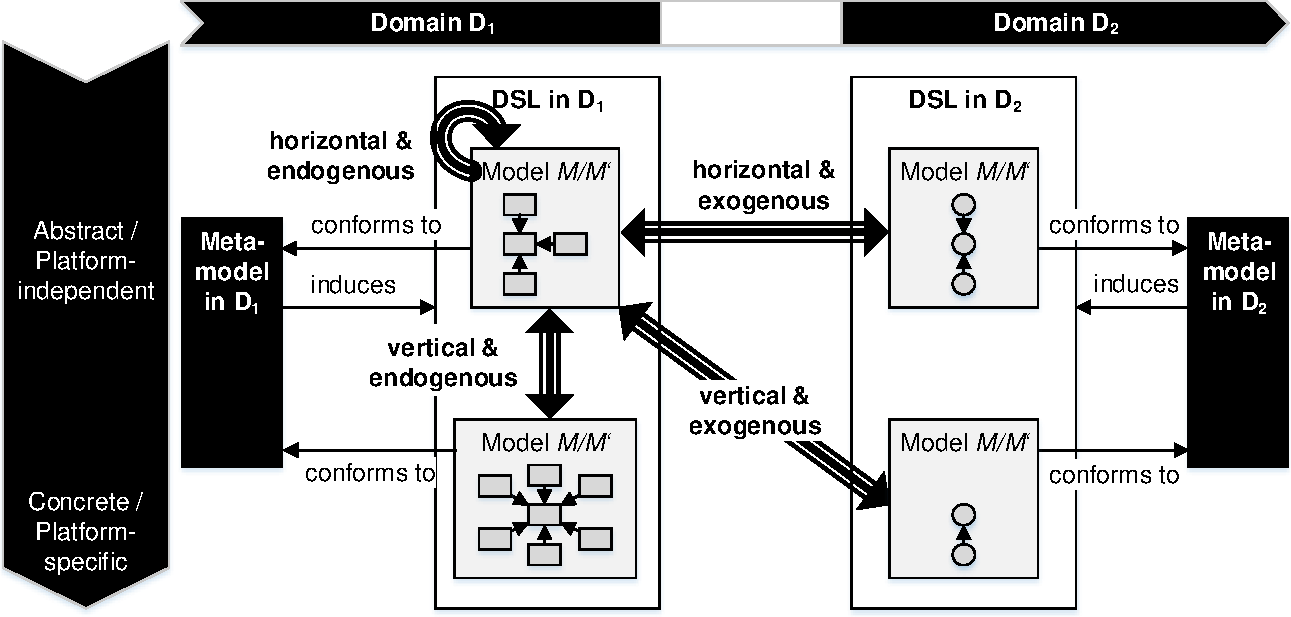
\includegraphics[width=\textwidth]{img/gen_intro/mt.pdf}
\end{center}
\caption{Classification of Model Transformations (Adaption from \cite{FAGT2})}
\label{fig:sec-gen-intro-mt:mt}
\end{figure}

\begin{figure}[!tb]
\begin{center}
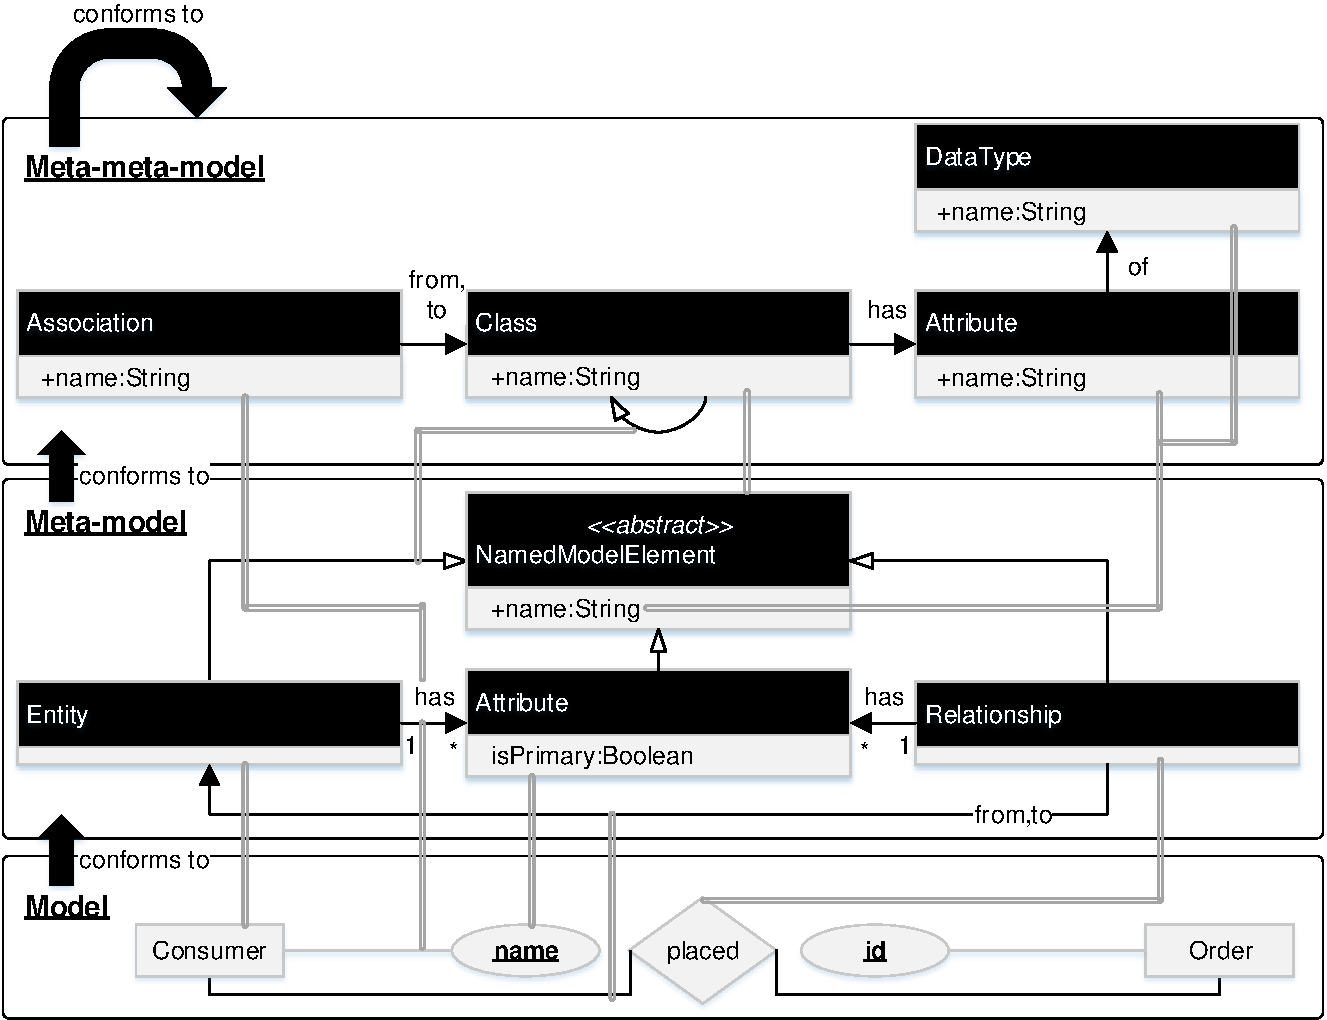
\includegraphics[width=.95\textwidth]{img/gen_intro/meta.pdf}
\end{center}
\caption{Different Layers of Meta-Modelling}
\label{fig:sec-gen-intro-mt:meta}
\end{figure}

Furthermore, DSLs $\Lang(D_1)$ and $\Lang(D_2)$ are each defined by a meta-model in the corresponding domain, i.e., $\Lang(D_1)$ ($\Lang(D_2)$) is induced by a meta-model in domain $D_1$ ($D_2$) (cf. \cref{fig:sec-gen-intro-mt:mt}).
The meta-model defines the concepts of the domain and their interrelationships that can be used in models.
In turn, $\Lang(D_1)$ ($\Lang(D_2)$) is the set of all models that conform to the meta-model in $D_1$ ($D_2$), i.e., the models only contain the concepts and interrelationships of the meta-model as model elements.
For example, we consider the DSL of entity-relationship diagrams in the domain where we want to reflect over the different entities of a system and their interrelationships.
The modelling language is defined by the meta-model in \cref{fig:sec-gen-intro-mt:meta}.
Entity-relationship diagrams may contain several \code{Entit}ies and directed \code{Relationship}s between them, i.e., each relationship is directed \code{from} an entity \code{to} an entity.  
Moreover, entities and relationships may have several \code{Attribute}s that may be primary keys (\code{isPrimary}).
By inheritance, each entity, relationship and attribute is a \code{NamedModelElement} and therefore, has a \code{name} of type \code{String}.
Note that the class \code{NamedModelElement} is declared as \code{<<abstract>>}, i.e., entity-relationship diagrams are not allowed to directly contain nodes of type \code{NamedModelElement} but only in the form of entities, relationships and attributes.
Therefore, the language of entity-relationship diagrams is given by all diagrams (models) that conform to the meta-model.
For example, the model in \cref{fig:sec-gen-intro-mt:meta} conforms to the meta-model.
\code{Consumer} and \code{Order} are \code{Entit}ies whereas \code{placed} is a \code{Relationship} \code{from} \code{Consumer} \code{to} \code{Order}.
Entity \code{Consumer} (\code{Order}) \code{has} a \code{name} (\code{id}) as \code{Attribute} which is marked as primary key (\code{isPrimary}=$\true$).

This view can also be applied to the meta-model where the language of meta-models is defined by a meta-meta-model.
Most meta-models can be expressed by means of the concepts of class diagrams that are given in excerpts by the meta-meta-model in \cref{fig:sec-gen-intro-mt:meta}.
Each meta-model may contain several \code{Class}es and \code{Association}s \code{from} classes \code{to} classes.
Furthermore, each class may have several \code{Attributes} \code{of} some \code{DataType} and with some \code{name} of type \code{String}.
Between two classes there may be an inheritance relationship.
For example, the meta-model in \cref{fig:sec-gen-intro-mt:meta} conforms to the meta-meta-model.
\code{Entity}, \code{Attribute} and \code{Relationship} are \code{Class}es that inherit from class \code{NamedModelElement}.
From class \code{Entity} to class \code{Attribute} there is an \code{Association} with \code{name} \code{has}.
The same is true for class \code{Relationship} and \code{Attribute}.
The class \code{Attribute} \code{has} an \code{Attribute} with \code{name} \code{isPrimary} \code{of} \code{DataType} \code{Boolean}.
Analogously, class \code{NamedModelElement} has an attribute of name \code{name} and of type \code{String}.
In turn, the language of meta-meta-models can be defined by a meta$^3$-model such that the meta-meta-models conform to the meta$^3$-model etc..
However, in order to have a closure over the ``conforms to'' relation, OMG proposes a three-layer hierarchy of meta-modelling, i.e., models, meta-models and meta-meta model, where the meta-meta-model is defined by (conforms to) itself (cf. Fig. 6 in \cite{Henderson-Sellers2013}).
Note that for the language of class diagrams, the meta-meta-model may directly serve as the meta-model which leads to only two layers of meta-modelling.

\begin{figure}[!tb]
\begin{center}
\begin{tikzpicture}[]
\fill (0,0) node[inner sep=1pt] (A) {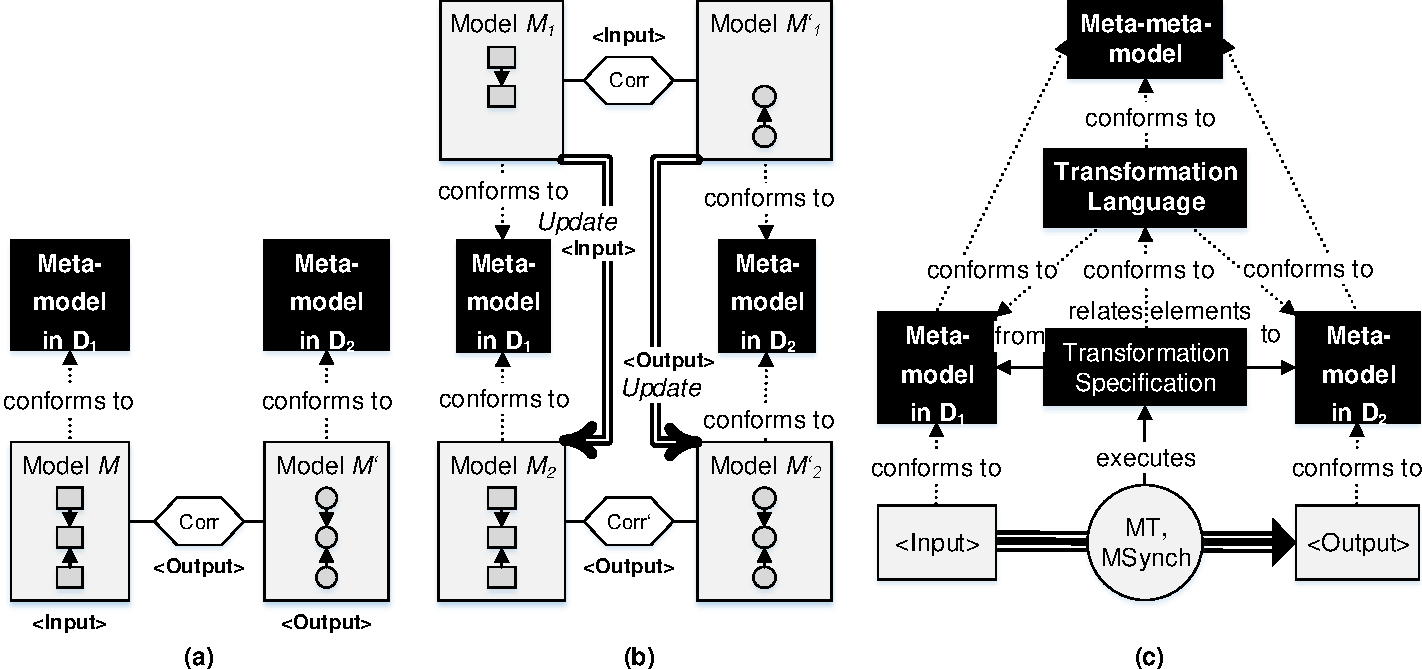
\includegraphics[width=\textwidth]{img/gen_intro/mt_msynch.pdf}};
\fill (-.8,1.2) node[inner sep=1pt] (B) {\small{$\delta$}};
\fill (.1,-.5) node[inner sep=1pt] (C) {\small{$\delta'$}};
\end{tikzpicture}
\end{center}
\caption{Setting of Model Transformations (a), Model Synchronisations (b) \& their Execution (c) (Adaption from \cite{FAGT2,Lucio2014})}
\label{fig:sec-gen-intro-msynch:mt_msynch}
\end{figure}

\cref{fig:sec-gen-intro-msynch:mt_msynch} (c) illustrates the execution of a model transformation that takes a source model $M \in \Lang(D_1)$ over the meta-model in source domain $D_1$ as input and outputs a target model $M' \in \Lang(D_2)$ over the meta-model in target domain $D_2$ together with a correspondence (\code{Corr}) which relates elements from $M$ to $M'$ as depicted in \cref{fig:sec-gen-intro-msynch:mt_msynch} (a).
The model transformation (MT) is performed by executing the model transformation specification.
The specification is defined based on the two meta-models in domains $D_1$ and $D_2$ and defines which model elements in $D_1$ should be transformed to which model elements in $D_2$ by relating (mapping) model elements from $D_1$ to $D_2$.
The transformation specification is expressed in (conforms to) a transformation language.
The transformation language contains (allows to express) the set of all conceivable mappings of model elements from $D_1$ to $D_2$.
Therefore, the transformation language conforms to the meta-models in domains $D_1$ and $D_2$ which in turn conform to a common meta-meta-model (cf. \cref{fig:sec-gen-intro-mt:meta}), i.e., the transformation language indirectly conforms to this meta-meta-model.
Although, both meta-models may conform to different meta-meta-models in general, the assumption of a common meta-meta-model of class diagrams is valid as already discussed.

Different model transformation approaches and tools \cite{HLG13+,Rose2014} do exist.
Beside model transformation by-example \cite{Kappel2012} where the transformation specification is generated from a given source model, target model and their correspondence, different types of transformation languages exist for explicitly specifying the transformation \cite{Guerra2013}, e.g., QVT \cite{QVT}, ATL \cite{Jouault200831}, triple graph grammars (TGGs) \cite{DBLP:journals/eceasst/AnjorinLS15} and ETL \cite{Kolovos2008}.
Different types of transformation languages may allow transformation specifications in textual or visual form and in declarative or operational manner \cite{tm13}.
While declarative transformation specifications focus on the specific mapping of model elements between domains, operational specifications additionally provide the concrete steps how the target model is derived from a source model, e.g., by providing the concrete order of traversing the model elements of the source model.
Furthermore, we distinguish between in-place model transformations and ``external" transformations where the source model is preserved by the transformation while the target model is constructed in parallel.
Moreover, model-to-model transformations are distinguished from model-to-text, text-to-model and text-to-text transformations.
However, note that any of these types of transformations can be simulated by ``external'' model-to-model transformations where the parallel target model is taken as output of an in-place transformation and text is parsed to (serialised from) a model before (after) executing the model-to-model transformation.
Therefore, we focus on ``external" model-to-model transformations based on TGGs that allow visual, declarative transformation specifications.
We review basic concepts and notions in \cref{sec-tgg,sec-mt-tgg}.
Beside the model-to-model transformation CD2RDBM from UML class diagrams to relational database models in \ref{sec-mt-tgg}, we present software transformations, i.e., text-to-(text)model transformations, from source code to visual models (or source code again) in \cref{sec-compl-software-trans}.
